\documentclass[aspectratio=169,11pt,handout]{beamer}
\usetheme{default}
\usefonttheme{professionalfonts}
\usepackage{lmodern}
\setbeamertemplate{navigation symbols}{}
\setbeamertemplate{footline}[frame number]
\setbeamercolor{frametitle}{fg=black}
\setbeamerfont{frametitle}{series=\bfseries}
\usepackage{amsmath,amssymb,mathtools}
\usepackage{booktabs}
\usepackage{graphicx}
\usepackage{tikz}
\usetikzlibrary{arrows.meta,positioning}
\graphicspath{{figs/}}
\setbeamertemplate{background}{\begin{tikzpicture}[remember picture,overlay]
  \node[anchor=north east,inner sep=0pt] at ([xshift=-4pt,yshift=-4pt]current page.north east) {
\includegraphics[height=0.95cm]{oxford_logo.png}};
\end{tikzpicture}}
\tikzset{testbox/.style={draw=#1!60!black,fill=#1!6,rounded corners=4pt,line width=0.8pt,inner sep=8pt,anchor=north},
  testttl/.style={fill=#1!60!black,text=white,rounded corners=3pt,font=\bfseries\small,inner sep=4pt}}
\newcommand{\Q}{\mathbb Q}
\newcommand{\PP}{\mathbb P}
\newcommand{\E}{\mathbb E}
\newcommand{\dd}{\mathrm d}
\newcommand{\ip}[2]{\langle #1,#2\rangle}
\newcommand{\yes}{{\color{green!50!black}\checkmark}}
\newcommand{\no}{{\color{red!70!black}$\times$}}
\newcommand{\approxm}{{\color{orange!80!black}$\sim$}}
\newcommand{\headline}[1]{{\large\bfseries #1}}
\newcommand{\cin}[1]{{\color{blue!70!black}#1}}
\newcommand{\cout}[1]{{\color{orange!85!black}#1}}
\newcommand{\slideref}[1]{\begin{tikzpicture}[remember picture,overlay]
  \node[anchor=south west,font=\tiny,text=gray,text width=0.8\paperwidth,align=left] at ([xshift=12pt,yshift=5pt]current page.south west) {#1};
\end{tikzpicture}}
\newcommand{\divider}[2]{\begin{frame}\vspace*{0.35\textheight}{\Huge #1}\\[0.6em]{\large\color{gray}#2}\end{frame}}
\tikzset{callout/.style={draw=red!70!black,text=red!70!black,fill=white,rounded corners,font=\footnotesize\bfseries,align=center,inner sep=3pt},
         calloutarrow/.style={red!70!black,thick,-{Latex}}}

\title{GROMM}
\subtitle{Generative Risk-neutral Option Market Models}
\author{Magnus Wiese$^{\dagger}$ \and Hans Buehler$^{*}$ \and Blanka Horvath$^{*}$}
\institute{$^{\dagger}$Independent researcher\\[0.3em] $^{*}$Mathematical Institute, University of Oxford}
\date{QuantMinds International 2026}

\begin{document}
\maketitle

\begin{frame}{Agenda}
\begin{enumerate}
\setlength{\itemsep}{0.9em}
\item \textbf{Why:} desks need dynamics, not just today's fit
\item \textbf{The model:} discrete local volatility (DLV), with an explicit risk-neutral drift
\item \textbf{Evidence:} S\&P~500, and the same arbitrage test against other generators
\item \textbf{Summary:} what GROMM does, and what it doesn't
\end{enumerate}
\end{frame}

\divider{Why}{desks need dynamics, not just today's fit}

% -------------------------------------------------------------------
\begin{frame}{What desks run today}
\textbf{Local-stochastic volatility (LSV)}
\[
  \sigma_{\mathrm{Dupire}}^2(T,K)=L(T,K)^2\;\E\bigl[V_T\mid S_T=K\bigr].
\]
\begin{itemize}
\item refitted every day $\Rightarrow$ modelling inconsistency
\item SV part calibrated, not estimated from how the surface moves
\end{itemize}
\vfill
\pause
\begin{alertblock}{GROMM}
The whole surface is the state: its dynamics are \textbf{estimated from history} and \textbf{arbitrage-free from one day to the next}.
\end{alertblock}
\slideref{Dupire (1994). Pricing with a smile; Guyon, Henry-Labord\`ere (2011). The smile calibration problem solved.}
\end{frame}

% ===================================================================
% A  WHY
% ===================================================================
\begin{frame}{The missing model}
\begin{center}
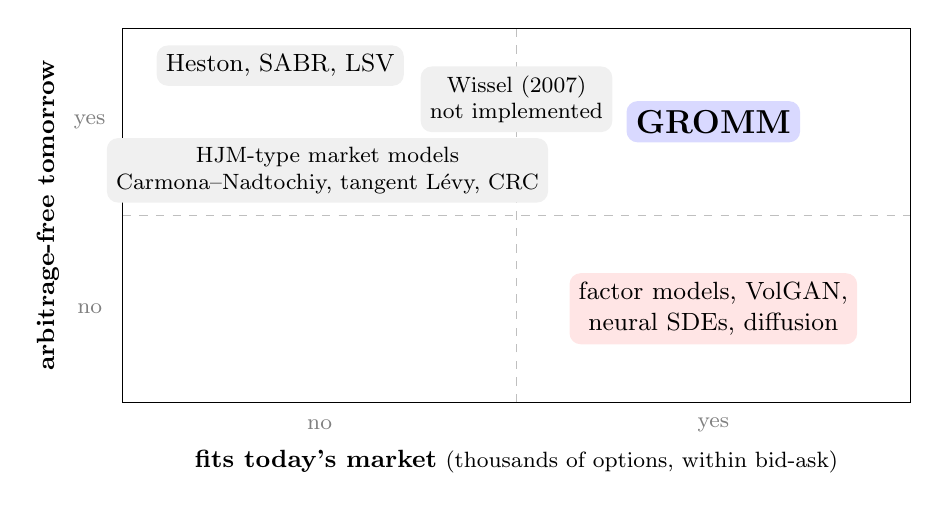
\begin{tikzpicture}[x=1cm,y=0.95cm,every node/.style={font=\small,align=center}]
  \draw (0,0) rectangle (10,5); \draw[gray!50,dashed] (5,0) -- (5,5); \draw[gray!50,dashed] (0,2.5) -- (10,2.5);
  \node[gray] at (2.5,-0.3) {\footnotesize no}; \node[gray] at (7.5,-0.3) {\footnotesize yes};
  \node[gray] at (-0.42,1.25) {\footnotesize no}; \node[gray] at (-0.42,3.75) {\footnotesize yes};
  \node at (5,-0.8) {\textbf{fits today's market}\ {\footnotesize(thousands of options, within bid-ask)}};
  \node[rotate=90] at (-0.95,2.5) {\textbf{arbitrage-free tomorrow}};
  \uncover<2->{\node[fill=gray!12,rounded corners] at (2.0,4.5) {Heston, SABR, LSV};}
  \uncover<3->{\node[fill=gray!12,rounded corners,font=\footnotesize] at (2.6,3.1) {HJM-type market models\\Carmona--Nadtochiy, tangent L\'evy, CRC};}
  \uncover<4->{\node[fill=red!10,rounded corners] at (7.5,1.25) {factor models, VolGAN,\\neural SDEs, diffusion};}
  \uncover<4->{\node[fill=gray!12,rounded corners,font=\footnotesize] at (5,4.05) {Wissel (2007)\\not implemented};}
  \uncover<5->{\node[fill=blue!15,rounded corners,font=\large\bfseries] at (7.5,3.75) {GROMM};}
\end{tikzpicture}
\end{center}
\vfill
\uncover<5->{\begin{center}
\textbf{Fits today's market and is arbitrage-free tomorrow, for every option at once.}
\end{center}}
{\footnotesize Schematic.}
\end{frame}

% -------------------------------------------------------------------
\begin{frame}{Why arbitrage-free dynamics matter}
Train any optimiser on a simulator, and it finds the simulator's arbitrage:
\begin{center}
\begin{tikzpicture}
  \node[anchor=south west,inner sep=0] (img) {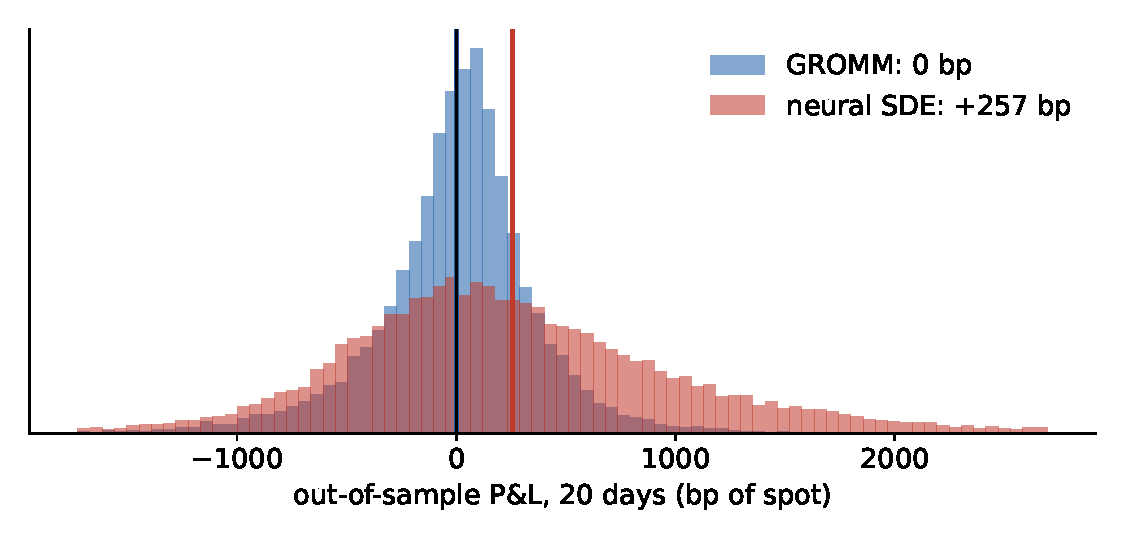
\includegraphics[width=\textwidth,height=.47\textheight,keepaspectratio]{opener_pnl.pdf}};
  \begin{scope}[x={(img.south east)},y={(img.north west)}]
    \node[callout] (c1) at (0.82,0.45) {neural SDE: +257\,bp\\from a model that should be fair};
    \draw[calloutarrow] (c1.west) -- (0.462,0.62);
    \node[callout,draw=blue!60!black,text=blue!60!black] (c2) at (0.13,0.45) {GROMM: 0,\\as it must be};
    \draw[calloutarrow,blue!60!black] (c2.east) -- (0.398,0.55);
  \end{scope}
\end{tikzpicture}
\end{center}
\vspace{-0.8em}
% {\footnotesize Fitted on half the simulated paths: the average price change of each of the 39 options on each of the 20 days (780 averages). Traded on the other half: buy or sell one of each option, following the sign, rebalanced daily. Same data and contracts for both models.}
{\footnotesize Out-of-sample P\&L of a buy-or-sell strategy, rebalanced daily: 39 options, 20 days.}
\vfill
\pause
\begin{itemize}
\item Any optimiser that trades the simulated options will find their arbitrage.
\item Costs hide it only if drift $<$ spread: no guarantee for a generic simulator.
\item \textbf{Cleaner: a simulator with an analytic $\Q$.}
\end{itemize}
\end{frame}

% ===================================================================
% B  THE IDEA
% ===================================================================
\divider{The model}{DLV, with an explicit drift}

\begin{frame}{The state: discrete local volatility (DLV)}
Fixed cash strikes $K^0<\dots<K^{N+1}$, fixed expiries $T_1<\dots<T_M$, call prices
$C^{j,i}=C(K^i,T_j)$.
\vfill
\[
  \Sigma^{j,i}
  =\frac{C^{j,i}-C^{j-1,i}}{(T_j-T_{j-1})\,\tfrac12\,(K^i)^2\,\Gamma^{j,i}}
  =\frac{\text{calendar spread}}{\text{butterfly}}
\]
\begin{center}
{\footnotesize discrete Dupire formula, $\Gamma$: discrete gamma (second difference in strike)}
\end{center}
\vfill
\pause
\begin{alertblock}{Key fact \normalfont(Buehler--Ryskin)}
\[
  \Sigma^{j,i}\geq 0\ \text{at every node}\quad\Longleftrightarrow\quad\text{no static arbitrage.}
\]
\end{alertblock}
So we model $\log\Sigma$: \textbf{any value is allowed}.
\slideref{Buehler, H., Ryskin, E.\ (2015). Discrete local volatility for large time steps.}
\end{frame}

% -------------------------------------------------------------------
\begin{frame}{The density recursion}
$q^j$: risk-neutral density of $S_{T_j}$ on the grid $=$ butterfly prices.
\vfill
\[
  \boxed{\;q^{j-1}=M^j\,q^j,\qquad M^j=I-\Omega_j\,\mathrm{diag}(\Sigma^j)\;}
\]
\begin{center}
{\footnotesize one implicit finite-difference step per expiry; $\Omega_j$: fixed tridiagonal matrix}
\end{center}
\vfill
\begin{center}
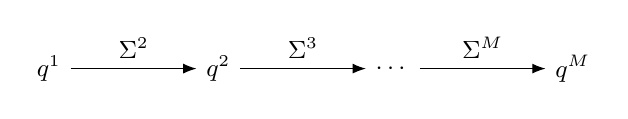
\begin{tikzpicture}[node distance=1.6cm, every node/.style={font=\small}]
  \node (q1) {$q^1$};
  \node[right=of q1] (q2) {$q^2$};
  \node[right=of q2] (qd) {$\cdots$};
  \node[right=of qd] (qM) {$q^M$};
  \draw[-{Latex}] (q1) -- node[above]{$\Sigma^2$} (q2);
  \draw[-{Latex}] (q2) -- node[above]{$\Sigma^3$} (qd);
  \draw[-{Latex}] (qd) -- node[above]{$\Sigma^M$} (qM);
\end{tikzpicture}
\end{center}
\vfill
\pause
\begin{center}
Front density $q^1$ $+$ any $\Sigma\ge0$ $\;\Longrightarrow\;$ every density, every price.
\end{center}
\end{frame}

% -------------------------------------------------------------------
\begin{frame}{Itô on the recursion}
\cin{\textbf{Input:}} the vol of DLV, any number of factors. \cout{\textbf{Unknown:}} the drift.
\[
  \frac{\dd\Sigma^{j}_t}{\Sigma^{j}_t}=\cout{\mu^j_t}\,\dd t+\cin{\xi^j_t}\,\dd W_t .
\]
\pause
\textbf{No arbitrage:} densities are butterflies, so they are martingales,
$\dd q^j_t=E^j_t\,\dd W_t$.
\pause
\vspace{-0.3em}
\[
  \dd q^{j-1}=M^j\,\dd q^j+(\dd M^j)\,q^j+\dd[M^j,q^j]
\]
\pause
\vspace{-0.6em}
\begin{columns}[T]
\column{.5\textwidth}
\centering\textbf{match $\dd W$}
\[
  E^j=(M^j)^{-1}\bigl(E^{j-1}+\Omega_jB^jq^j\bigr)
\]
{\footnotesize one tridiagonal solve}
\column{.5\textwidth}
\centering\textbf{set $\dd t$ to zero}
\[
  \boxed{\;\cout{\mu^{j,i}}=-\ip{\cin{\xi^{j,i}}}{\eta^{j,i}},\quad \eta=\frac{E}{q}\;}
\]
{\footnotesize node by node}
\end{columns}
\vfill
\pause
\slideref{Drift restriction: Wissel (2007), in local implied volatilities; continuum: Carmona, Nadtochiy (2009).}
\end{frame}

\begin{frame}{Where the recursion starts: the front density}
\vspace{0.5em}
Front density $q^1$: \textbf{any martingale on the grid} with
\[
  \boxed{\;\dd q^{1}_t=\cin{E^{1}_t}\,\dd W_t\;},\qquad
  q^1_t\ge0,\quad \mathbf 1^\top q^1_t=1,\qquad
  q^1_{T_1}=e_J\ \text{for some node } J .
\]
Spot is a read-off, the mean of the front density:
\(
  X_t=K^\top q^1_t,\ X_{T_1}=K^J .
\)
\begin{center}
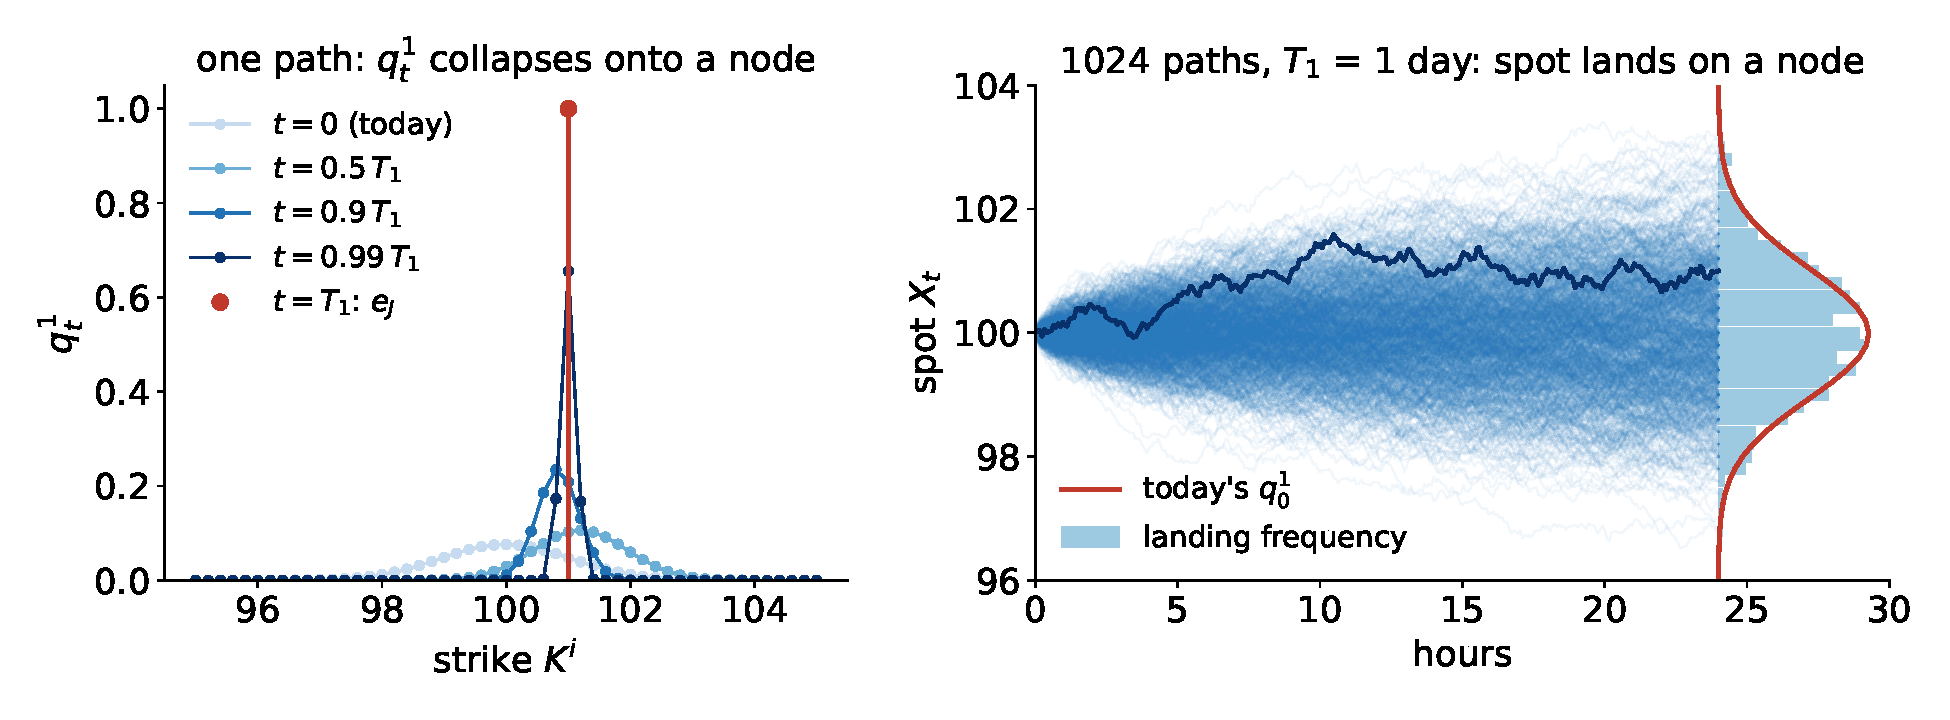
\includegraphics[width=.95\textwidth]{front_quantile_1d.pdf}
\end{center}
\end{frame}

\begin{frame}{No arbitrage, and the model exists}
\begin{alertblock}{Proposition (drift restriction)}
\[
  \text{every } q^j \text{ is a martingale}
  \qquad\Longleftrightarrow\qquad
  \cout{\mu^{j,i}}=-\ip{\cin{\xi^{j,i}}}{\eta^{j,i}}\ \text{ at every node}
\]
\end{alertblock}
\vfill
\begin{alertblock}{Theorem (existence)}
If the vol of vol $\cin{\xi}$ is locally Lipschitz and bounded, GROMM has a unique solution: every $\Sigma^{j,i}$ stays finite and positive, and at each expiry spot settles on a node and the model continues.
\end{alertblock}
\vfill
\begin{itemize}
\item any number of factors, no conditions on the wings
\item any network decoder with bounded output (tanh, clip) qualifies
\end{itemize}
\end{frame}

% -------------------------------------------------------------------
\begin{frame}{Estimating the dynamics from history}
\textbf{AR(1)} per node, same contract from day $d$ to $d+1$, with $L=\log\Sigma$:
\[
  L_{d+1}=a+b\,L_d+{\color{gray}\varepsilon_d}
  \qquad\Longrightarrow\qquad
  \mu^{\PP}_{\text{emp}}=252\,\bigl[a+(b-1)L_d\bigr]+\tfrac12|\cin{\xi}|^2
\]
\vspace{-0.3em}
\textbf{Loadings} from the residuals: factor 1 is the spot shock (regression), the rest is PCA:
\[
  {\color{gray}\varepsilon_d}\approx\sum_{f}\ell_f\,Z^f_d,
  \qquad
  \cin{\xi^f}=\sqrt{252}\,\ell_f
\]
\vspace{-0.3em}
\textbf{Drifts:} $\Q$ (pricing) is computed; $\PP$ (risk) adds a market price of risk $\theta$:
\[
  \cout{\mu^\Q}=-\ip{\cin{\xi}}{\eta},
  \qquad
  \mu^\PP=\cout{\mu^\Q}+\cin{\xi}\,\theta
\]
\vfill
\begin{center}
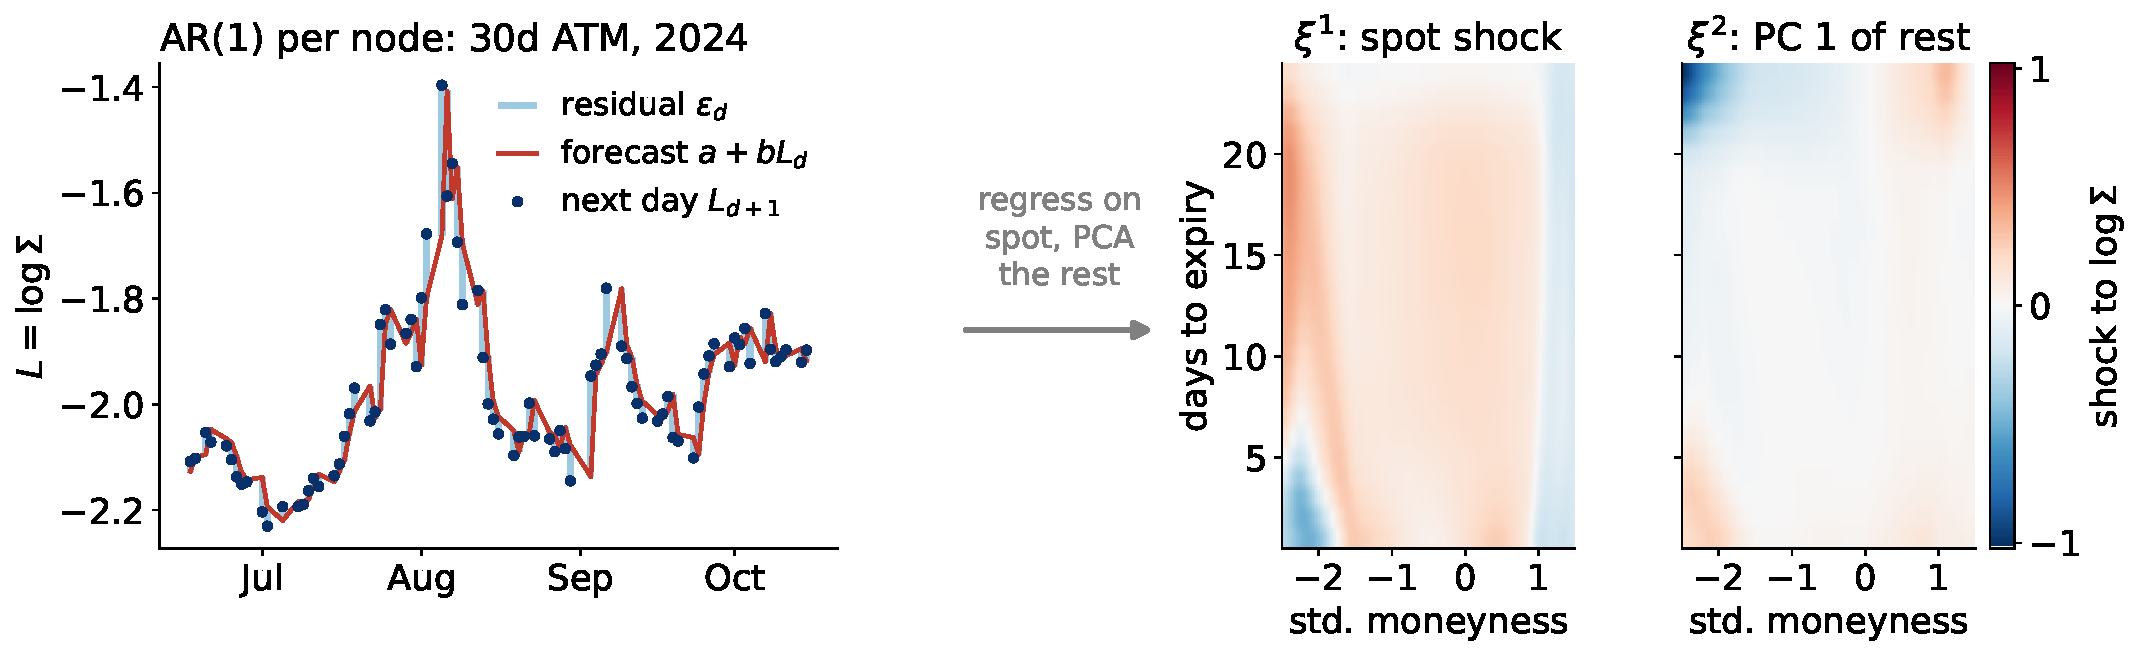
\includegraphics[width=\textwidth,height=.42\textheight,keepaspectratio]{est_pipeline.pdf}
\end{center}
\end{frame}

% ===================================================================
% C  EVIDENCE
% ===================================================================
\divider{Evidence}{fit $\cdot$ test $\cdot$ S\&P~500 $\cdot$ head-to-head}

\begin{frame}{Day 0: fitting SPX}
\begin{center}
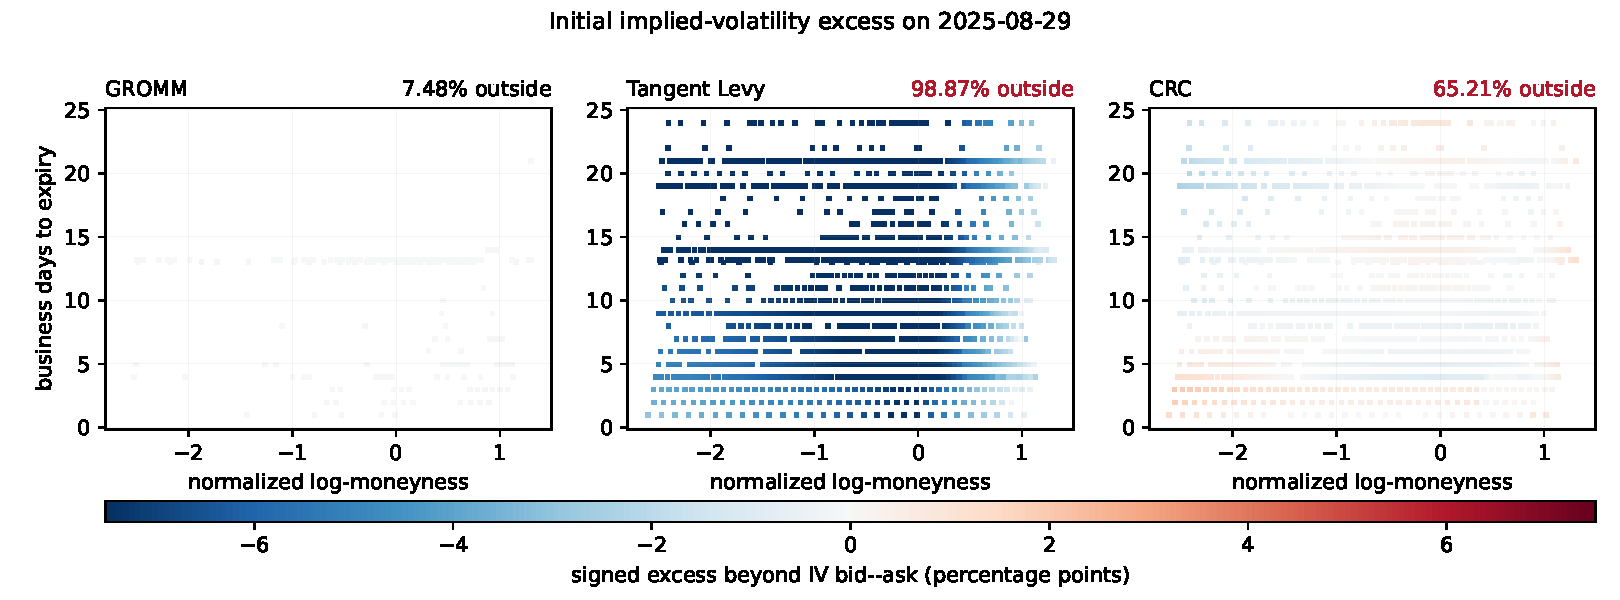
\includegraphics[width=.92\textwidth,trim=0 51 0 0,clip]{initial_fit_iv_errors.pdf}\\[1.2em]
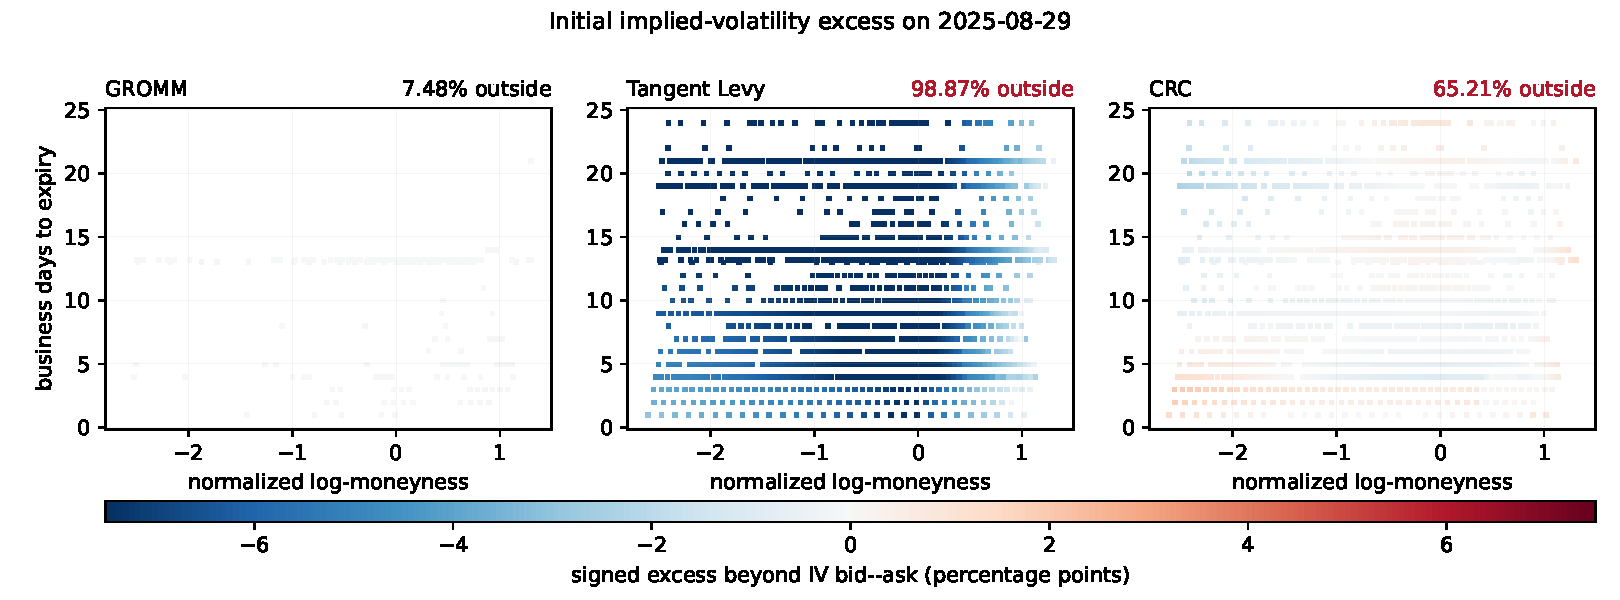
\includegraphics[width=.92\textwidth,trim=0 0 0 237,clip]{initial_fit_iv_errors.pdf}
\end{center}
\vfill
\begin{center}
\headline{97\%}\ of 2.2M SPX quotes (2022--25) inside bid-ask
\end{center}
\end{frame}

% -------------------------------------------------------------------
\begin{frame}{How to test for dynamic arbitrage: the BHW test}
\begin{center}
Under $\Q$ every traded price is a martingale:\quad $\E_t\bigl[\Delta C_t\bigr]=0,\qquad \Delta C_t=C_{t+1}-C_t$.
\end{center}
\vspace{0.6em}
\begin{center}
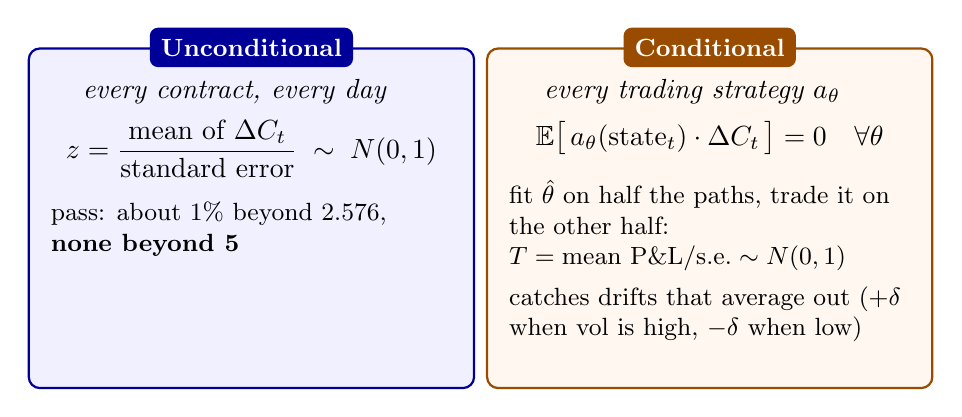
\begin{tikzpicture}
  \node[testbox=blue] (u) at (-0.24\textwidth,0) {\begin{minipage}[t][3.75cm][t]{0.42\textwidth}
    \vspace{0.3em}\textit{every contract, every day}\\[0.5em]
    \centering$\displaystyle z=\frac{\text{mean of }\Delta C_t}{\text{standard error}}\;\sim\;N(0,1)$\\[0.8em]
    \raggedright\small pass: about 1\% beyond 2.576,\\ \textbf{none beyond 5}
  \end{minipage}};
  \node[testttl=blue] at (u.north) {Unconditional};
  \node[testbox=orange] (c) at (0.24\textwidth,0) {\begin{minipage}[t][3.75cm][t]{0.42\textwidth}
    \vspace{0.3em}\textit{every trading strategy $a_\theta$}\\[0.5em]
    \centering$\displaystyle \E\bigl[\,a_\theta(\text{state}_t)\cdot\Delta C_t\,\bigr]=0\quad\forall\theta$\\[0.8em]
    \raggedright\small fit $\hat\theta$ on half the paths, trade it on the other half:
    $T=\text{mean P\&L}/\text{s.e.}\sim N(0,1)$\\[0.4em]
    catches drifts that average out ($+\delta$ when vol is high, $-\delta$ when low)
  \end{minipage}};
  \node[testttl=orange] at (c.north) {Conditional};
\end{tikzpicture}
\end{center}
\end{frame}

% -------------------------------------------------------------------
\begin{frame}{SPX: GROMM passes, and the test has power}
\begin{columns}[T]
\column{.5\textwidth}
\textbf{Full grid:} 5{,}001 instruments, 62{,}569 tests
\vspace{0.6em}

\begin{tabular}{@{}lcc@{}}
\toprule
 & expected & GROMM \\
\midrule
beyond 2.576 & 626 & 635 \\
beyond 5 & 0 & 0 \\
conditional $T$ & $N(0,1)$ & 0.84 \\
\bottomrule
\end{tabular}
\column{.48\textwidth}
\textbf{Power check:} 570 instruments
\vspace{0.6em}

\begin{tabular}{@{}lcc@{}}
\toprule
 & max $|z|$ & beyond 5 \\
\midrule
GROMM under $\Q$ & 2.7--3.7 & 0 \\
GROMM under $\PP$ & 342 & 570 \\
CRC under $\Q$ & 140 & 320 \\
\bottomrule
\end{tabular}
\end{columns}
\vfill
\begin{itemize}
\item under $\Q$: as many exceedances as chance predicts
\item under $\PP$ (risk premia) and for CRC (generalised Bates): rejected everywhere
\end{itemize}
\slideref{5{,}001 instruments $=$ 25 daily expiries $\times$ 200 strikes $+$ spot. Tests $=$ (instrument, day) pairs live and near the money on enough of 100{,}000 paths.}
\end{frame}


% -------------------------------------------------------------------
\begin{frame}{Head-to-head: same data, same BHW test}
\begin{center}
\begin{tikzpicture}
  \node[anchor=south west,inner sep=0] (img) {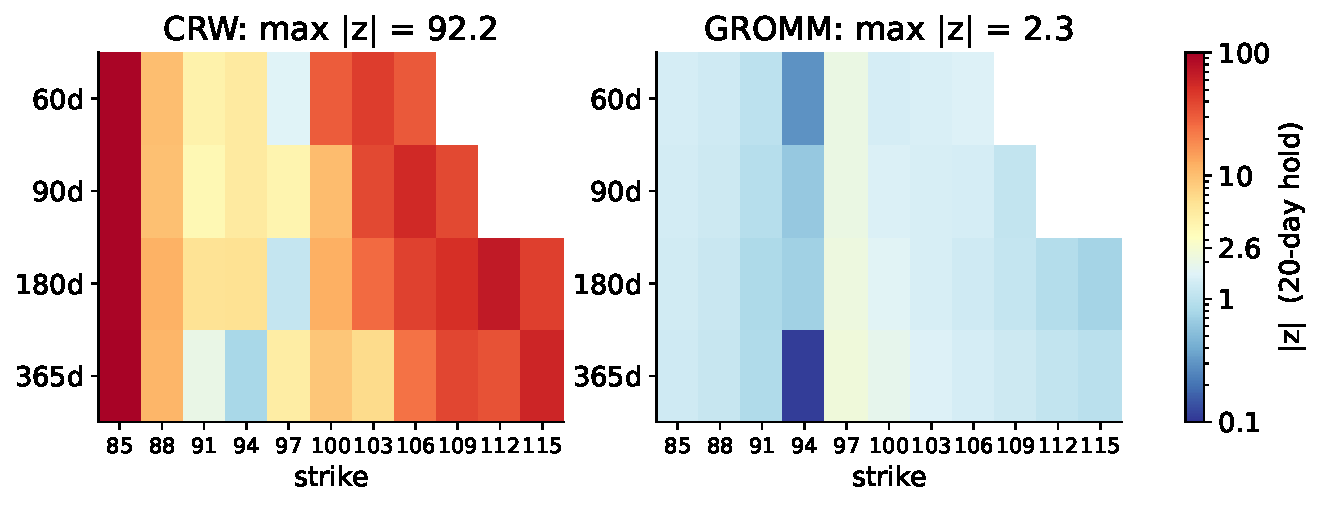
\includegraphics[width=\textwidth,height=.44\textheight,keepaspectratio]{zmap.pdf}};
  \begin{scope}[x={(img.south east)},y={(img.north west)}]
    \node[callout,anchor=east,overlay] (c) at (-0.06,0.52) {red $=$\\predictable drift};
    \draw[calloutarrow,overlay] (c.east) -- (0.09,0.52);
  \end{scope}
\end{tikzpicture}
\end{center}
\vspace{0.3em}
\begin{center}\small
\begin{tabular}{@{}lccc@{}}
\toprule
 & max $|z|$, 20-day hold & daily tests beyond 5 & tests \\
\midrule
neural SDE & 92.2 & 320 & 724\\
GROMM & 2.3 & 0 & 780\\
exact Heston (control) & 1.9 & 0 & 723\\
\bottomrule
\end{tabular}
\end{center}
\slideref{Heston-SLV benchmark and trained neural SDE of Cohen, Reisinger, Wang (2023); GROMM fitted to the same data,
rank 3 $=$ the neural SDE's 3 Brownian motions; same start state, 39 contracts, 20 days, 48{,}000 path pairs.}
\end{frame}

% -------------------------------------------------------------------
\begin{frame}{Deep hedging: no free lunch under GROMM}
\centering
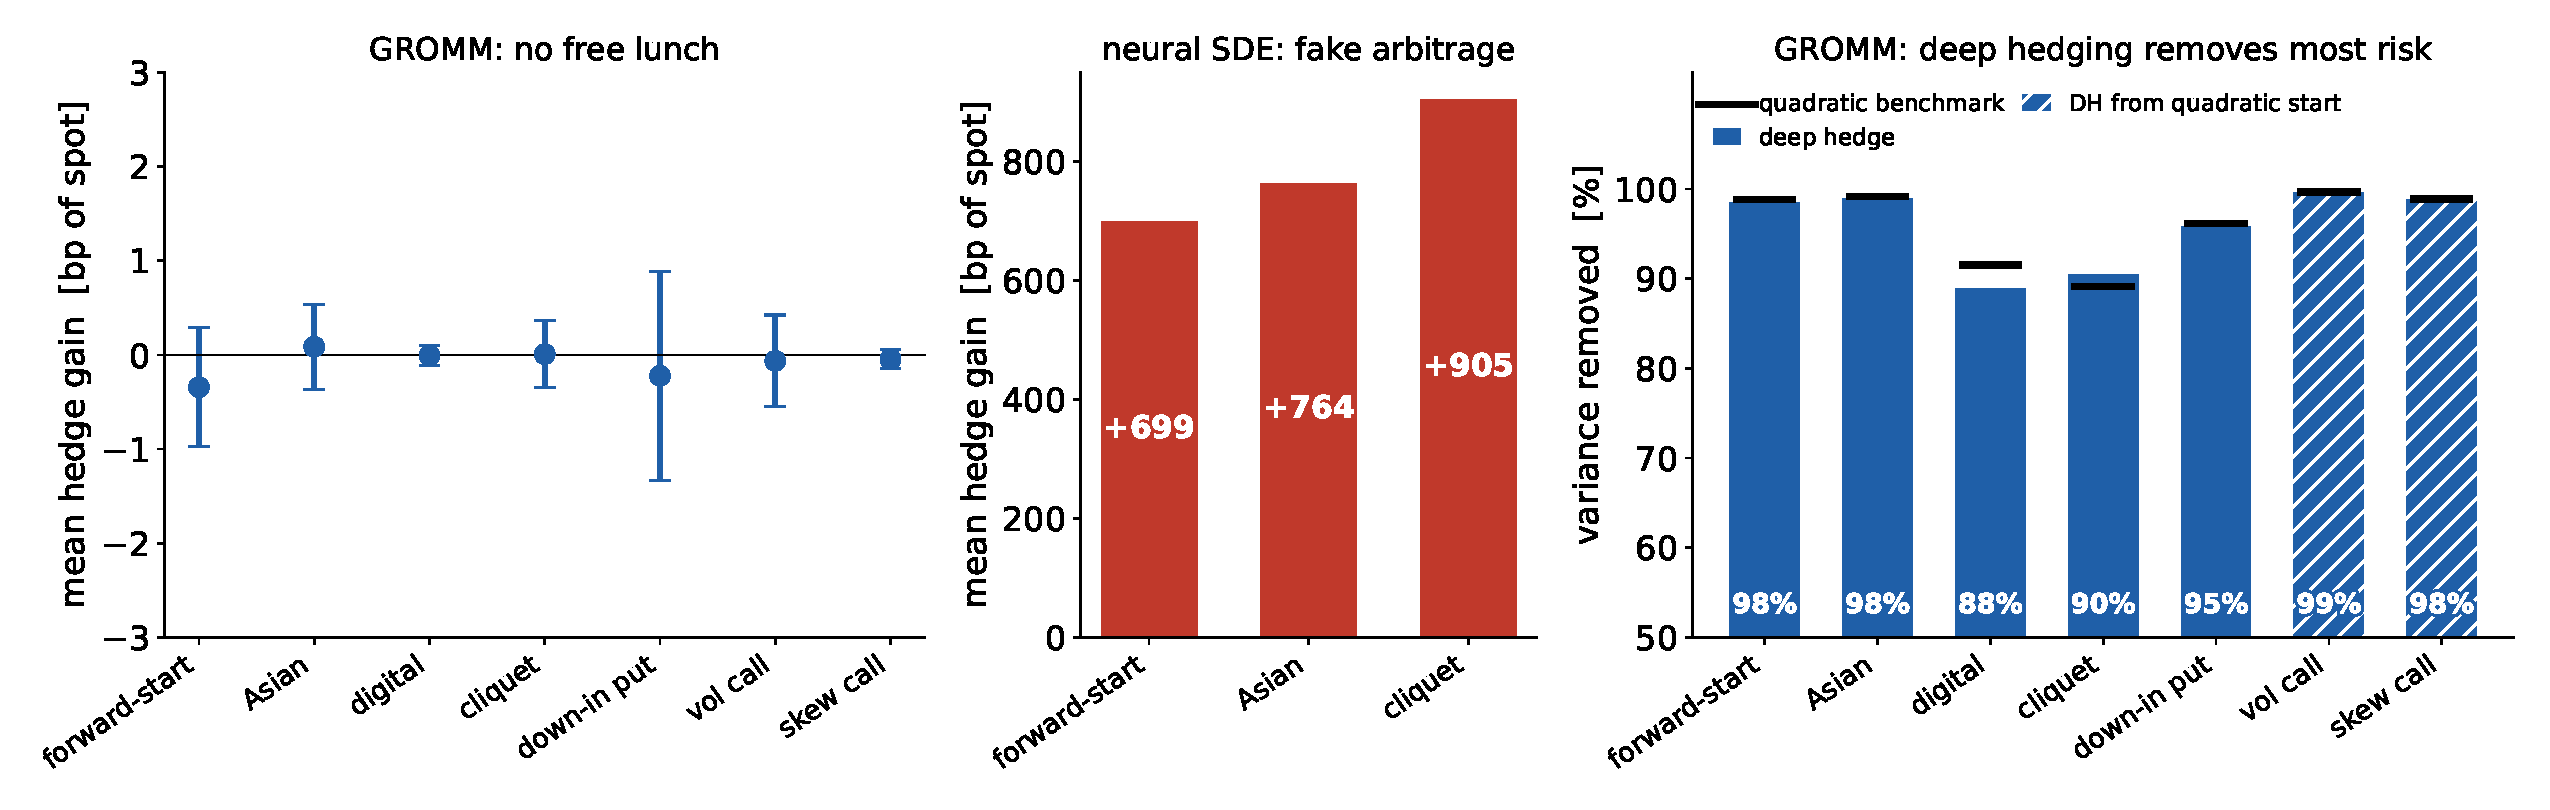
\includegraphics[width=\linewidth]{figs/dh_summary.pdf}
\vspace{-0.4em}
\[
  \text{hedge gain } G=\sum_t \delta_t\cdot\Delta C_t,
  \qquad
  \text{no arbitrage}\;\Longrightarrow\;\E_\Q[G]=0
\]
\slideref{GROMM rank 3 and neural SDE on the Heston-SLV benchmark; 20 days; spot $+$ 3 options; $\lambda=100$ with spot $=1$; error bars $\pm2$ s.e.; quadratic benchmark $=$ least-squares hedge. Small networks on an Apple M1 Pro laptop; not tuned for performance.}
\end{frame}

% ===================================================================
% D  CLOSE
% ===================================================================
\divider{Summary}{what GROMM does, and what it doesn't}

\begin{frame}{What GROMM does, and what it doesn't (yet)}
\begin{columns}[T]
\column{.48\textwidth}
\textbf{Does}
\begin{itemize}
\item explicit $\Q$ for every option on the grid
\item no static and no dynamic arbitrage, by construction
\item 97\% of S\&P~500 quotes inside bid-ask, including the next-day expiry
\item $\PP$ and $\Q$ from one state
\item fast: one tridiagonal solve per factor and expiry
\end{itemize}
\column{.48\textwidth}
\textbf{Doesn't (yet)}
\begin{itemize}
\item vol of vol is estimated once from history: it does not change with the market state
\item continuous paths: no jumps
\end{itemize}
\end{columns}
\end{frame}

% -------------------------------------------------------------------
\begin{frame}{Takeaways}
\begin{enumerate}
\item \textbf{State $=$ discrete local volatility (DLV):} static arbitrage is impossible by construction.
\item \textbf{Itô on the density recursion:} an explicit drift, node by node. Dynamic arbitrage is impossible by construction.
\item \textbf{On SPX:} 97\% inside bid-ask, and 62{,}569 BHW arbitrage tests passed. Other generators fail the same test.
\end{enumerate}
\vfill
\begin{center}
arXiv:2610.16732
\end{center}
\end{frame}

\begin{frame}
\vspace*{0.35\textheight}{\Huge Please ask questions}\\[0.6em]
{\large\color{gray}arXiv:2610.16732}
\end{frame}

% ===================================================================
\appendix
\begin{frame}{Appendix: our front, spot as a quantile of a Brownian motion}
Spot at the front expiry lands on a grid node, drawn with the spot factor $W^1$:
\[
  X_{T_1}=F^{-1}\!\bigl(\Phi(W^1_{T_1}/\sqrt{T_1})\bigr),\qquad F:\ \text{CDF of today's } q^1 .
\]
$W^1$ is revealed over time. With $a_i=\Phi^{-1}(q^{1,0}+\dots+q^{1,i})$,
\[
  q^{1,i}_t=\Q\bigl(X_{T_1}=K^i\mid\mathcal F_t\bigr)=\Phi(z_i)-\Phi(z_{i-1}),\qquad
  z_i=\frac{\sqrt{T_1}\,a_i-W^1_t}{\sqrt{T_1-t}} .
\]
\[
  \boxed{\;\dd q^{1,i}_t=\cin{E^{1,i}_t}\,\dd W^1_t,\qquad
  \cin{E^{1,i}_t}=\frac{\phi(z_{i-1})-\phi(z_i)}{\sqrt{T_1-t}}\;}
\]
\vfill
\begin{itemize}
\item a martingale by construction, in closed form: the front density vol $E^1$
\item at $T_1$ spot settles on a node
\end{itemize}
\end{frame}

\begin{frame}{Appendix: who has tried (1/2), generative and ML simulators}
\scriptsize
\resizebox{\textwidth}{!}{%
\begin{tabular}{@{}llccl@{}}
\toprule
 & model & no static arb. & explicit $\Q$ & grid (expiries $\times$ strikes) \\
\midrule
Wiese, Bai, Wood, Buehler (2019) & DLV, PCA and GAN & \yes{} on grid & \no & $8\times4$ \\
Wiese et al.\ (2021) & DLV latent flow & \yes{} on grid & \no & $9\times4$ per asset \\
Medvedev, Wang (2022) & LSTM / ConvLSTM on IVs & \no & \no & \\
Cohen, Reisinger, Wang (2023) & neural SDE & \yes{} on grid & \approxm{} penalty & $5\times11$ \\
Cont, Vuleti\'c (2023) & IV factors, path reweighting & \approxm & \no & fixed IV grid \\
Zhang, Li, Zhang (2023) & VAE and neural surface & \approxm & \no & $14\times11$ \\
Ning, Jaimungal, Zhang, Bergeron (2023) & VAE to pricing-model parameters & \yes & \no & parametric \\
Choudhary, Jaimungal, Bergeron (2024) & functional PCA, neural SDE & \no & \no & $17\times11$ \\
Vuleti\'c, Cont (2024) & VolGAN & \approxm & \no & \\
Jin, Agarwal (2025) & conditional diffusion & \approxm & \no & $9\times9$ \\
Brooks et al.\ (2026) & penalised VAE, latent flow & \approxm & \no & $32\times16$ \\
Hao, Ji (2026) & diffusion with refinement & \approxm & \no & $15\times17$ \\
Han et al.\ (2026) & sequential diffusion & \approxm & \no & $11\times9$ \\
Yang, Wang, Zhang, Li (2026) & diffusion across equities & \approxm & \no & $11\times9$ per stock \\
Fran\c{c}ois et al.\ (2026) & five-factor IV with SPX & \approxm & \no & \\
Buchegger, Gonon (2026) & latent diffusion & \approxm & \no & \\
\midrule
\textbf{GROMM} & \textbf{stochastic DLV} & \yes & \yes & $\mathbf{25\times200}$ \\
\bottomrule
\end{tabular}}
\vfill
{\footnotesize \approxm: approximate (penalties, reweighting, measured violation rates). Full classification: paper, Appendix.}
\end{frame}

\begin{frame}{Appendix: who has tried (2/2), market models}
\small
\resizebox{\textwidth}{!}{%
\begin{tabular}{@{}llccl@{}}
\toprule
 & model & no static arb. & explicit $\Q$ & fit / scale \\
\midrule
Cont, da Fonseca (2002); Fengler, H\"ardle, Villa (2003) & IV factor models & \no & \no & empirical $\PP$ \\
Wissel (2007) & option lattice, local implied volatilities & \yes & \yes{} drift, existence & not implemented \\
Schweizer, Wissel (2008) & local implied volatility & \yes & \yes{} theory & one expiry \\
Carmona, Nadtochiy (2009) & local-volatility codebook & --- & drift only & no existence proof \\
Carmona, Ma, Nadtochiy (2017) & tangent L\'evy & \yes & \yes & 98.9\% outside bid-ask$^{\ast}$ \\
Gambara, Teichmann (2021) & consistent recalibration (Bates) & \yes & \approxm{} fails as calibrated & 65.2\% outside bid-ask$^{\ast}$ \\
Buehler, Horvath, Kratsios, Wiese (2026) & DySANOS & \yes & \approxm{} 48 options & SPX \\
\midrule
\textbf{GROMM} & \textbf{stochastic DLV} & \yes & \yes{} \textbf{5{,}000 options} & \textbf{97\% inside bid-ask} \\
\bottomrule
\end{tabular}}
\vfill
{\footnotesize $^{\ast}$our implementation, SPX on 29 Aug 2025.}
\end{frame}

\end{document}
